%----------Appendices-----------------------------------------------------------
\appendix
% ---------------
% Appendix A
\section{Appendix: Criticality Distribution}\label{sec:subsec_6.1}

The approach to calculating the measure of criticality was explained in Section~\ref{sec:criticality} of this paper. In more detail, Equations~\eqref{eq:q_value}, \eqref{eq:max_q_value}, and \eqref{eq:variance} are used to obtain a single value that represents the criticality measure for a single observation. While performing 10 experiments of 1000 episodes each, criticality measures were collected. Based on the number of appearances of particular criticality values, the distribution shown in Figure~\ref{fig:crit_distribution} was generated.

\paragraph{Density-Function Approach for Criticality Visualisation}

For the analysis and visualisation of criticality metrics recorded throughout the experiments, the density-function approach was employed. The value of criticality, being a variance of Q-values, is a continuous variable that spans a wide range of values. To observe the behaviour of models via criticality distribution, the \texttt{Seaborn} library, an extension of \texttt{Matplotlib}, was utilized. This made the visualisation smooth and interpretable. Specifically, for estimating the probability density function of criticality, \texttt{Kernel Density Estimation (KDE)} was employed.

A common and widely used method to visualise the distribution of a continuous variable is the histogram~\cite{kde2018}. The principle of the histogram involves splitting the range of continuous data into a discrete number of bins and then counting the number of samples within each bin. When applied to criticality values, the histogram approach divides the data into discrete intervals and displays the occurrence counts for each interval. However, this approach has several limitations:

\begin{enumerate}
    \item \textbf{Sensitivity to Bin Size:} Choosing a larger bin size can lead to excessive generalisation and oversimplification of the graph. Conversely, smaller bin intervals can introduce noise and complicate result interpretation.
    \item \textbf{Discontinuity:} Producing a stepped output, histograms cannot accurately convey patterns of continuous values such as criticality.
    \item \textbf{Information Loss:} The discretisation of continuous values inevitably leads to the loss of valuable information about fluctuations in the explored variable.
\end{enumerate}

Given these limitations, histograms are not an optimal method for representing criticality as a continuous value. Instead, the \texttt{Kernel Density Estimation (KDE)} method was employed.

\paragraph{Kernel Density Estimation for Criticality Visualisation}

Unlike histograms, KDE does not rely on discrete intervals; rather, it produces a smooth curve by approximating the distribution of the variable. This method helps to generate graphs of continuous distributions while preserving the original complex patterns~\cite{kde2018}.

By applying a kernel function (usually a Gaussian function) to every data point and summing the resultant functions, KDE produces a smooth estimate of the density function. KDE is regulated by two key parameters: \textit{bandwidth} and \textit{kernel function type}.

\begin{enumerate}
    \item \textbf{Bandwidth:} The bandwidth parameter characterises the width of the kernel function application interval and thus determines the smoothness of the final graph. A wider bandwidth results in a smoother function with fewer details, while a smaller bandwidth preserves details but can also introduce noise to the estimated graph~\cite{chen2017tutorialkerneldensityestimation}.

    \item \textbf{Kernel Function:} The type of kernel function defines the influence of each data point on the final curve. For its symmetric and smooth properties, the Gaussian distribution is commonly used as the kernel function.
\end{enumerate}

\paragraph{Implementation of KDE for Criticality Visualisation}

To utilise KDE for criticality visualisation, the \texttt{Seaborn} library implementation was used. \texttt{Seaborn} is a Python library designed as an extension of \texttt{Matplotlib}~\cite{seaborn2021}. The \texttt{sns.kdeplot()} function was employed for visualising the criticality variable. This function created smooth density curves for criticality values, as represented in Figure~\ref{fig:crit_distribution}. The criticality values were recorded over a total of 10,000 episodes of model evaluation. To enhance the visualisation, a logarithmic scale was applied to the y-axis, representing the density of particular criticality values.

\begin{figure}[H]
    \centering
    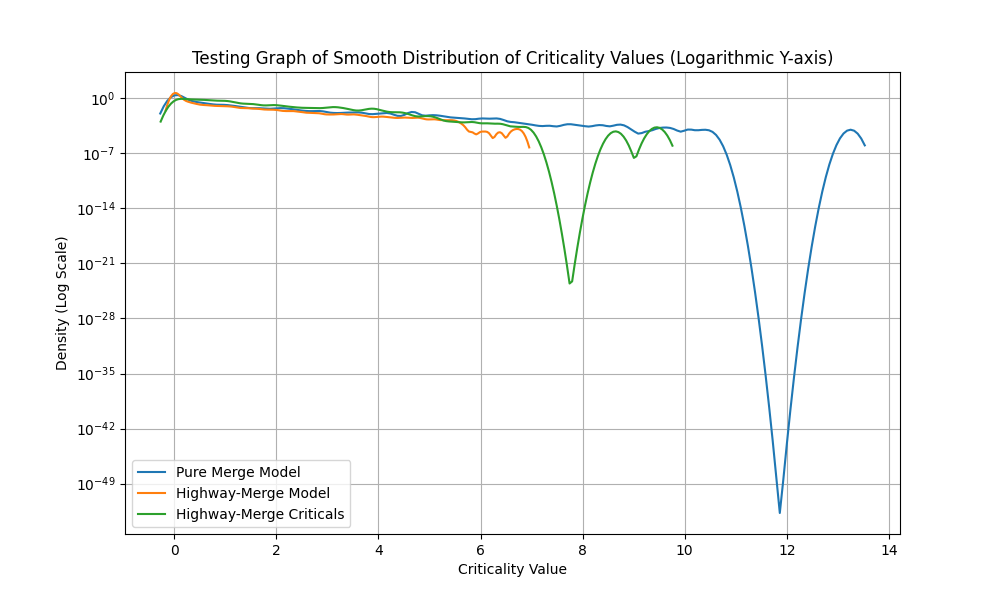
\includegraphics[width=\textwidth]{images/Criticality_distribution.png}
    \caption{Combined distribution of criticality values throughout episodes for every model.}
    \label{fig:crit_distribution}
\end{figure}

Observing Figure~\ref{fig:crit_distribution}, differences in the criticality range of explored models can be noticed. The widest range of values is owned by \texttt{Pure Merge Model}. The biggest values observed in the criticality set of this model are approximately 13-13.5. If comparing this with the highest values of different models (\texttt{Highway-Merge Criticals}), numbers are getting down rapidly: 8.5-9.5. Analysing a wider range of criticality in the pure RL model it can be deduced that it tends to observe and/or initiate states where one of its actions plays the role of a single safe solution. Referring to TL models, the \texttt{Highway-Merge Model} performed with the statistics where the highest criticality values were in an interval of 6.5-7.

Although graphs show density function lines ending at particular points, there is also a form of graphs to be explored. As described previously, KDE approximates the probability density function of a variable by summing the chosen kernel function at each point of appearance. If observing the pattern of a blue graph on the interval 12-14 and the green graph on the interval 7.5-10 we can see multiple original Gaussian functions overlapping. However, those kinds of peaks represent single values and outliers of an overall set. To prove that, Figure~\ref{fig:test_kde} was constructed, where an additional single value was appended to the criticality values array for the \texttt{Highway-Merge Criticals} model. Thus the additional value 11 appeared as a Gaussian function centered at 11.

\begin{figure}[H]
    \centering
    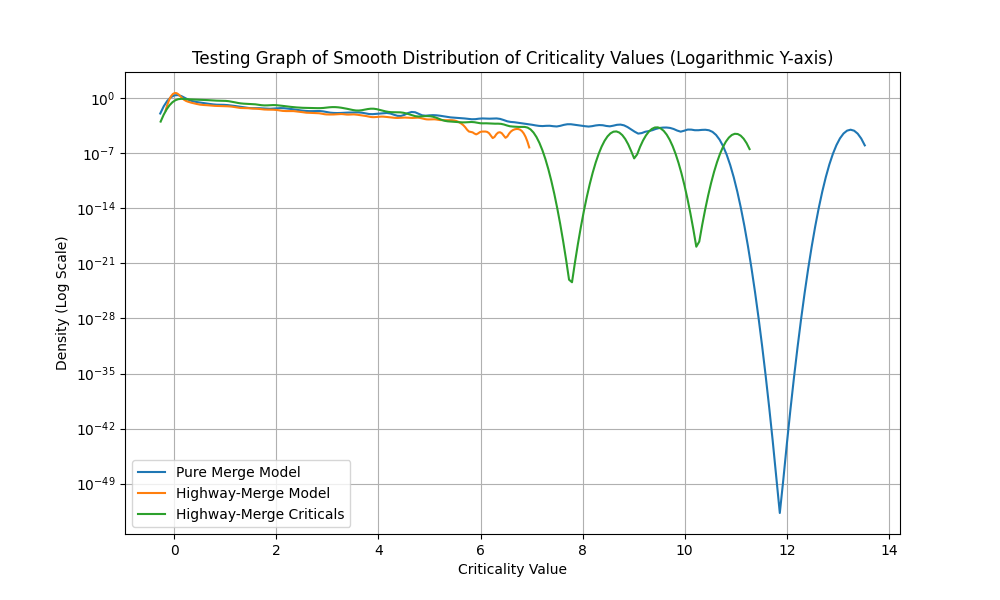
\includegraphics[width=\textwidth]{images/Test_kde.png}
    \caption{Test criticality distribution graph, created to show the principles of KDE}
    \label{fig:test_kde}
\end{figure}

Based on this KDE principle exploration, values higher than 10.5 for \texttt{Pure Merge Model} and higher than 7.0 for \texttt{Highway-Merge Model} are single-value outliers. 

In general, it can be noticed that TL models are better at handling criticality, and are prone to get into less critical scenarios rather than pure RL models.

